\documentclass{article}
\usepackage[left=0.5in,top=0.5in,right=0.5in,bottom=0.5in]{geometry}
\usepackage[english]{babel}
\usepackage[utf8]{inputenc}
\usepackage[table]{xcolor}
\usepackage{amssymb,amsmath,amsthm}
\usepackage{changepage,threeparttable}
\usepackage{booktabs,multirow}
\usepackage{graphicx}
\usepackage{soul}
\graphicspath{{./images/}}
\def\F#1{\(#1\)}
\def\C{\(\text{\textdegree}\)}
\title{Lab 10: Earth's Magnetic Field}
\author{Philip Kim}
\date{\today}
\begin{document}
\maketitle
\vspace*{-1cm}
\begin{enumerate}
  \item Record the initial dip angle \F{\theta_0} = \boxed{36\text{\textdegree}}
  \item Set source to 4V.
  \begin{table}[!htp]\centering
    \begin{tabular}{|c|c|c|c|c|c|c|}\hline
      \multicolumn{7}{|c|}{\textbf{Table 1: Earth's Measurement of Magnetic Field}} \\\hline
      Resistance&20\(\Omega \)&40\(\Omega \)&75\(\Omega \)&150\(\Omega \)&180\(\Omega \)&200\(\Omega \)\\\hline
      Current i&0.122A&0.0733A&0.0442A&0.0256A&0.0212A&0.0182A\\\hline
      Dip Angle \F{\Theta_i}&-71\C&-49\C&-14\C&6\C&12\C&15\C\\\hline
      Calculated \F{B_i}&1.44e-4&8.65e-5&5.22e-5&3.02e-5&2.50e-5&2.15e-5\\\hline
      \F{tan (\theta_i)}&-2.90&-1.15&-0.25&0.11&0.21&0.27\\\hline
    \end{tabular}
  \end{table}
  \item Record the Helmholtz coil radius: R = 9.75cm \(\rightarrow \boxed{0.0975m}\)
  \item Record the Helmholtz coil number of turns: N = \F{\boxed{128}}
  \item Calculations: (\F{B_i=\frac{8N_{\mu_0}I_i}{R\sqrt{125}},~where~\mu_0=4\pi\times10^{-7}Tm/A},~\(\tan(36\text{\textdegree})=\frac{B_H}{B_V} = 0.727\))
  \begin{itemize}
    \item Plot \F{tan \theta_i} vs \F{B_i} with straight line. Deduce the values of \F{B_V} and \F{B_H} from the graph.
    \item \F{B_V = B_E\cdot cos (\theta_0) \rightarrow\ B_E\cdot cos (36\text{\textdegree})=\boxed{0.809T}}
    \item \F{B_H = B_E\cdot sin (\theta_0) \rightarrow\ B_E\cdot sin (36\text{\textdegree})=\boxed{0.588T}}
    \item Calculate \F{B_E = \frac{B_H}{sin (36\text{\textdegree})} \rightarrow\ \frac{0.588}{sin (36\text{\textdegree})}=\boxed{1.0004T}}
    \item Lookup value of \F{B_E = \frac{3.02e-5}{0.11 -\ 0.727} = \boxed{-4.89\times10^{-5}T}}
    \item \F{Slope = \frac{1}{-4.89\times10^{-5}T} \rightarrow\ \boxed{-2.04\times10^4T}}
  \end{itemize}
\end{enumerate}
\begin{center}
  \subsection*{Graph}
  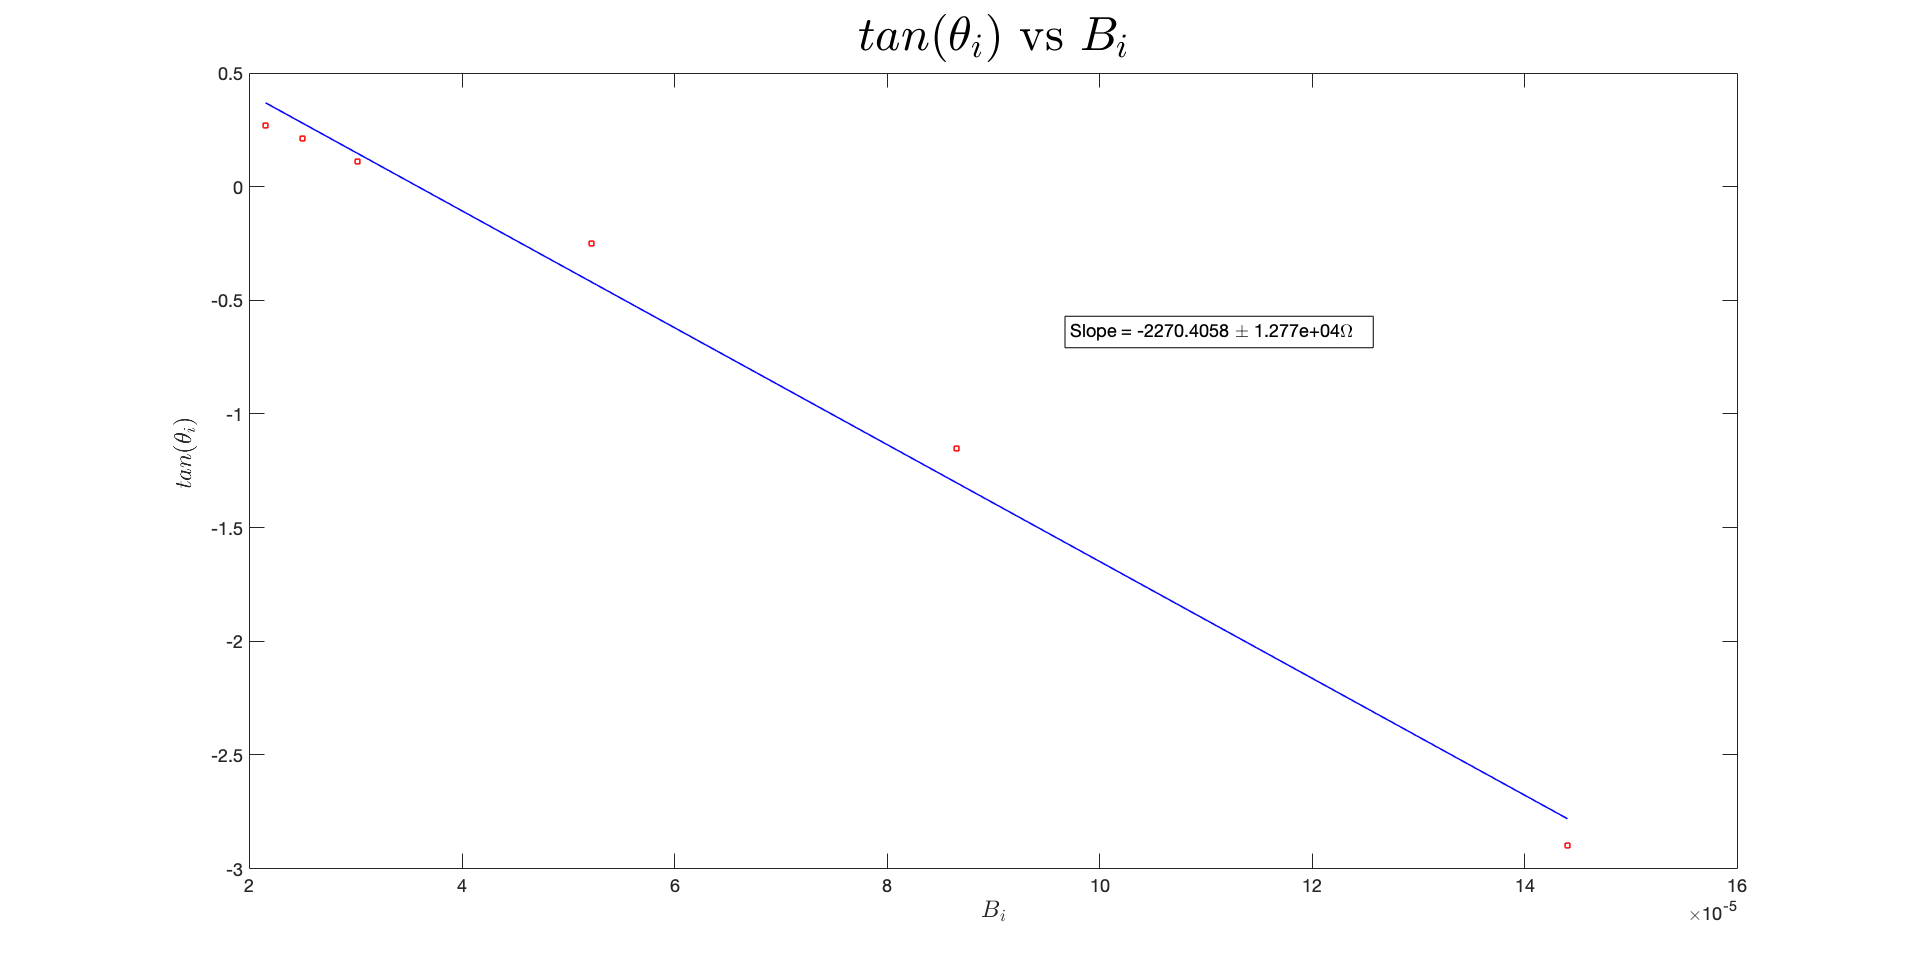
\includegraphics[scale=0.25]{graph.png}
\end{center}
\end{document}
